\section{Einleitung}\raggedbottom 

\subsection{Motivation}

Das Sammelkarten Spiel ''Magic The Gathering'' von Wizards of the Coast wird weltweit von etwa 20 Millionen  Spielern gespielt \footnote{\cite{GuardianMagicReport}}. 
Für das Spiel erscheinen regelmäßig neue Sätze an Karten. Spieler stellen aus der großen Auswahl an Karten eine eigene Auwahl zusammen, die als ''Deck'' bezeichnet wird, mit der sie gegen andere Spieler spielen.
Während des Spiels ziehen Spieler Karten von ihrem Deck und spielen diese strategisch in Zügen aus, mit dem Ziel, die ''Lebenspunkte'' des anderen Spielers von 20 auf 0 zu bringen.

Der Hersteller des Spieles betreibt eine große Turnierszene, in der Spieler aus aller Welt teilnehmen können.
In diesem Turniersystem sind über eine Millionen Spieler registriert und über 65000 \footnote{\cite[~p.7]{HasbroQ1Financial}}  nehmen in großen Turnieren mit mehreren tausend Spielern teil.
Diese großen Turniere werden im Internet live auf \url{twitch.tv/magic} übertragen. Besonders die Pro Tour, ein Event, zu dem die Spieler sich über andere Turniere qualifizieren müssen, lockt mehrere 10000 Zuschauer an \footnote{\cite{TwitchStat}}.

In diesen Liveübertragungen ist es nicht möglich, den Text auf Karten zu lesen (siehe Abbildung \ref{fig:screenshot}). Dieser ist jedoch für das Spiel sehr relevant, da, ohne den Text zu kennen, der Spielverlauf nicht nachvollzogen werden kann. 
Will ein Zuschauer verstehen, was im Spiel passiert, muss dieser die Karten anhand der Bildern auf ihnen identifizieren und auswendig wissen, was auf der jeweiligen Karte steht.

Dies ist besonders für neue Spieler und nach dem Erscheinen von neuen Karten ein Problem. 

Das Ziel dieser Arbeit soll es sein, ein Verfahren zu finden, welches automatisiert Karten in Videobildern finden und diese dann erkennen kann.
Dieses Verfahren soll als Grundlage für eine Anwendung dienen, welche automatisch Karten in einem Livevideo findet und den Kartentext bzw. ein Bild der Karte in lesbarer Qualität anzeigt.
Dadurch soll es neuen Spielern ermöglicht werden, Turniere zu verfolgen und den Spielverlauf zu verstehen.

\begin{figure}[h]
    \centering
		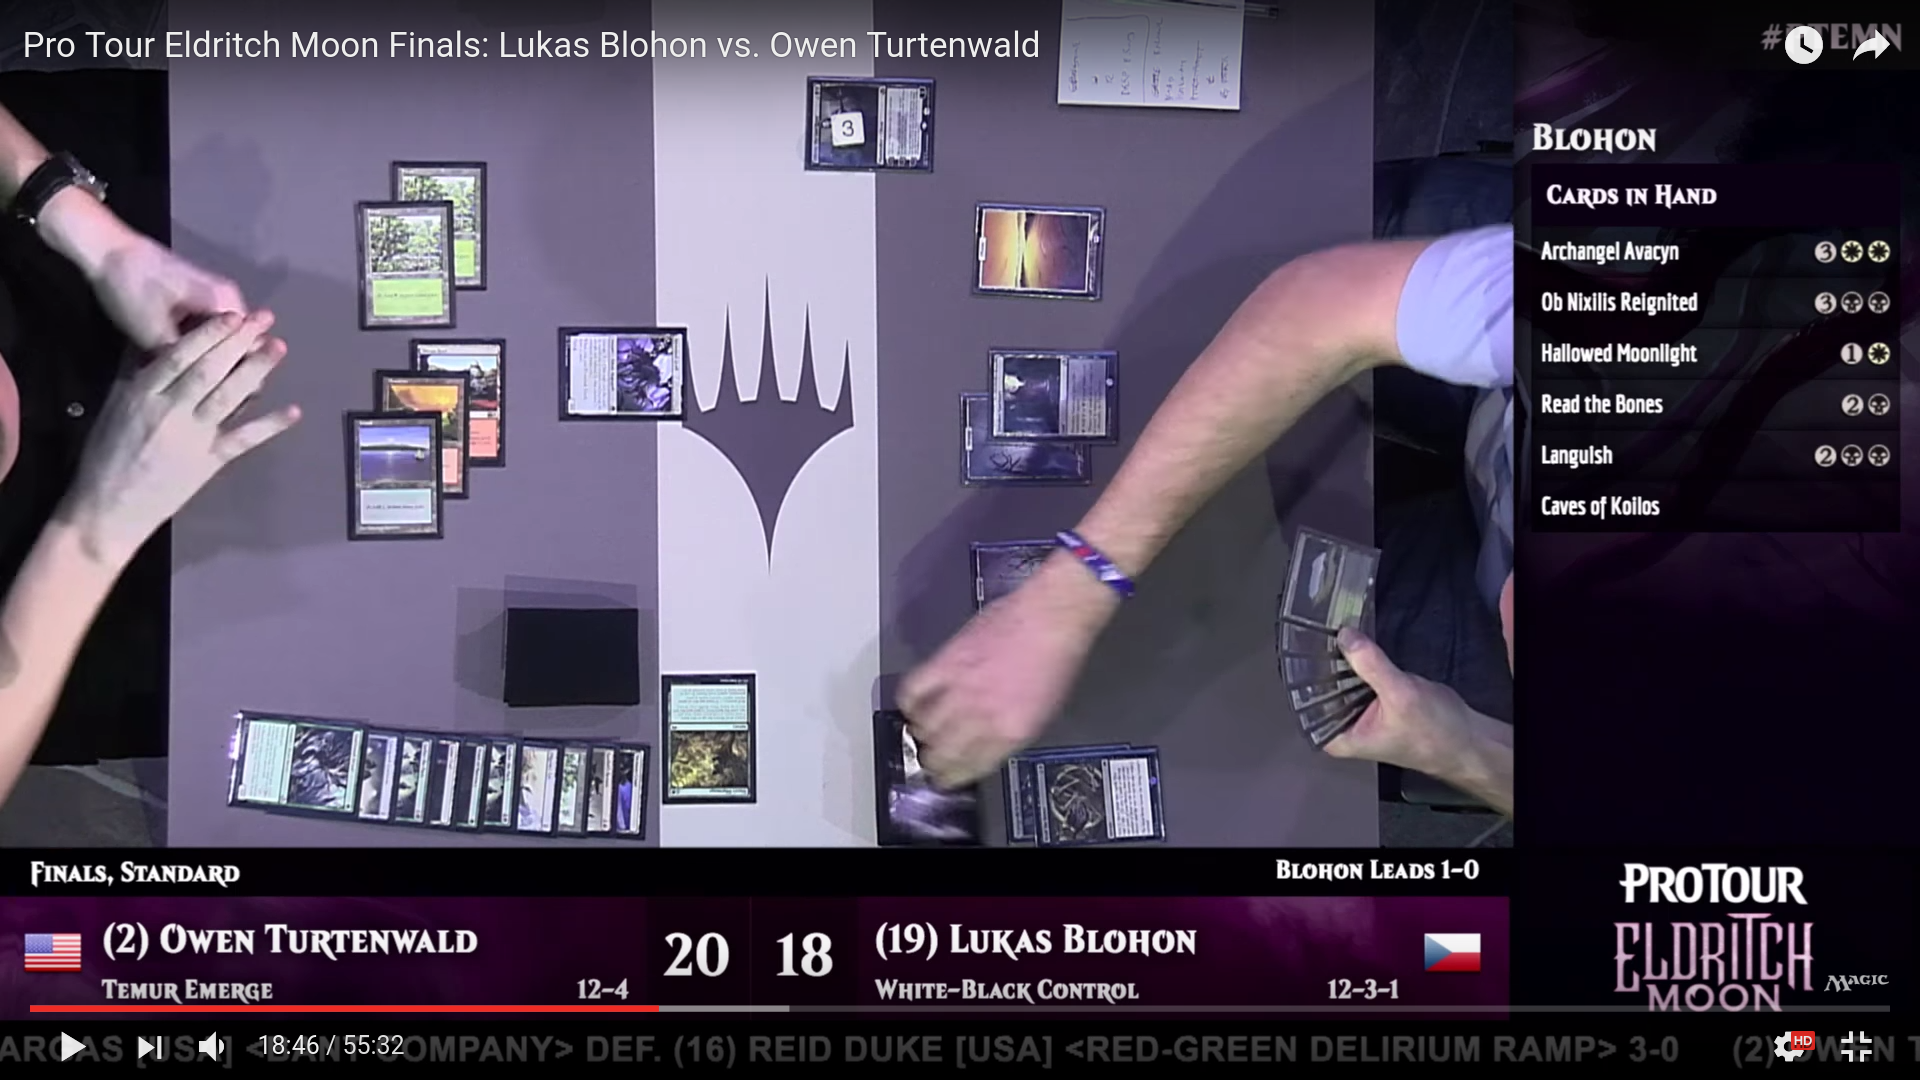
\includegraphics[scale=0.2]{bilder/screenshot.png}
    	\caption{Ein Bild aus den Videoaufnahmen.}
\label{fig:screenshot}
\end{figure}

\subsection{Aufbau} 

In dieser Arbeit werden zuerst grundlegende Methoden der Bildverarbeitung erläutert. Aufbauend auf diesen werden drei Verfahren betrachtet, die sogenannte Merkmale in einem Bild finden. Mit diesen Merkmalen können Objekte in verschiedenen Bildern wiedererkannt werden.


Es wird ein Klassifikator vorgestellt, der anhand der Merkmale, die diese Verfahren finden, Bilder von Karten klassifizieren kann.

Es wird ein Trainingsdatensatz erstellt, aus dem die Merkmale der einzelnen Karten berechnet werden. Dieser Trainingsdatensatz enthält Kartenbilder, die auf der offiziellen Seite des Herstellers zu finden sind.
 Zudem wird ein Testdatensatz erstellt. Dieser besteht aus Bildern von Karten, die aus Videos der Liveübertragung herausgeschnitten wurden. Zudem wird der Testdatensatz künstlich, mit häufig auftretenden Veränderungen, wie Rotation, erweitert. 

In einem Auswertungsteil wird die Erkennungsrate des Klassifikators mithilfe des Testdatensatzes analysiert.

Anschließend wird ein Verfahren vorgestellt, welches automatisch Karten in einem Videobild lokalisieren kann. In Verbindung mit dem Klassifikator können Karten so automatisch in einem Video gefunden und erkannt werden.
Dies wird genutzt, um den Trainingsdatensatz automatisch zu erweitern.
Es wird untersucht, ob diese Erweiterung zu einer besseren Erkennungsrate führt.
